\documentclass[11pt]{amsart}
\usepackage[margin=1in]{geometry}                % See geometry.pdf to learn the layout options. There are lots.
\geometry{letterpaper}                   % ... or a4paper or a5paper or ... 
%\geometry{landscape}                % Activate for for rotated page geometry
%\usepackage[parfill]{parskip}    % Activate to begin paragraphs with an empty line rather than an indent
\usepackage{graphicx}
\usepackage{amssymb}
\usepackage{epstopdf}
\DeclareGraphicsRule{.tif}{png}{.png}{`convert #1 `dirname #1`/`basename #1 .tif`.png}

\title{Math 228b, Spring 2014, homework 1}
\author{Jake Edman}
\date{}                                           % Activate to display a given date or no date
\begin{document}
\maketitle
\section{Introduction}
This homework set is primarily concerned with solving the heat equation (or diffusion equation) in one spatial dimension along a bounded interval [0,1], with the solution fixed at 0 at both ends. The heat equation is one of the simplest PDEs, so it seems like a good choice for the first homework. 
The first part of the assignment deals with the simplest form of this equation, 
\begin{equation} 
u_t =u_{xx} 
\end{equation} 
while later parts introduce a diffusivity coefficient $\alpha$, which may depend on $x$, so the equation becomes
\begin{equation} 
u_t = \alpha(x) u_{xx}
\end{equation} 


\section{solve $u_t = u_{xx}$ on [0,1] with I.C. $u(x,0)= \sin(\pi x)$}

For the first part of the homework, I will the following numerical scheme: 
\begin{equation} 
u_j^{n+1} = u_j^n + \lambda (u_{j+1}^n - 2u_j^n + u_{j-1}^n)
\end{equation}\label{scheme} 
where $\lambda = k/h^2$, and $k$ and $h$ are the time and space discretization, respectively.  Boundary conditions are applied at the end of each time step, by setting $u(0,(nk)) = u(j_{max}h, nk) = 0$.


\subsection{solution for $h=k=1/10$; show instability. }
Figure \ref{u1} depicts the solution at $t=1$.  This solution is clearly very bad, and unstable. Heat should diffuse out along the domain, away from the initial maximum at $x=0.5$, and because there are no sources or sinks in the domain, it should simply flatten out to zero over time, and never become negative.  Additionally, the solution should be symmetrical along the x axis; the initial condition and boundary conditions are symmetric, and there are no sources or sinks to break the symmetry. The solution depicted in figure \ref{u1} changes sign as we move along the x axis, and is not symmetric, which must arise from  numerical instability. Instability is expected; in class, we showed that this scheme is stable for $\lambda \equiv \frac{k}{h^2} \le \frac{1}{2}$, and in this case $\lambda = 10$. 

\begin{figure}[t]
\begin{center} 
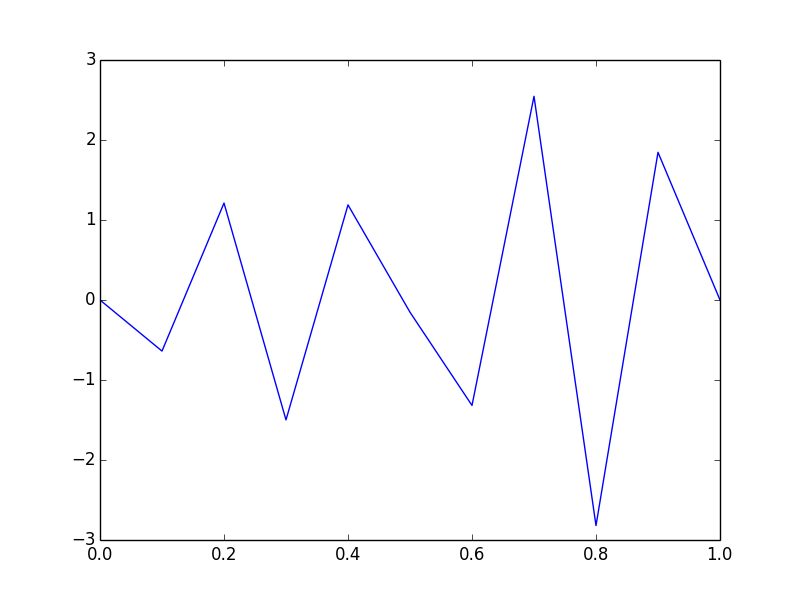
\includegraphics[width=5in,angle=0]{u1.pdf}
\caption{The solution to $u_t = u_{xx}$ with  $h=k=1/10$ }
\label{u1} 
\end{center}
\end{figure}
  
\subsection{solution for $h=1/10$, $k=1/200$; show stability.}
The solid blue line in figure \ref{u2} depicts the solution at $t=1$. Unlike the solution depicted in figure \ref{u1}, this solution appears stable, because it is smooth, nonnegative, and symmetric. It is behaving as we would expect the heat equation should, diffusing heat outward from the local maximum and gently flattening out over time. Nothing is growing out of control. We expect this stability, because $\lambda = 1/2$ in this case. 

\begin{figure}[t]
\begin{center} 
\includegraphics[width=5in,angle=0]{u1_2_conv.pdf}
\caption{The solution to $u_t = u_{xx}$ with $\lambda = 1/2$ for a range of meshes.}
\label{u2} 
\end{center}
\end{figure}

\subsection{solution for $\lambda = 1/6$, and compare order of convergence with $\lambda = 1/2$ } 

\begin{figure}[t]
\begin{center} 
\includegraphics[width=5in,angle=0]{u1_6_conv.pdf}
\caption{The solution to $u_t = u_{xx}$ with  $\lambda =1/6$ for a range of meshes.  }
\label{u16} 
\end{center}
\end{figure}

The dashed green line in figure \ref{u2} depicts the solution at $t=1$ for $\lambda =1/6$. This solution is clearly different than the one given by $\lambda =1/2$, but is it `better'? 

In class, we showed that truncation error is minimized for $\lambda = 1/6$;  the truncation error is defined as $\tau^k_h = u^{k}_h - u_{exact}$ where the superscript $u_h^k$ refer to the solution on a grid defined by space and  time discretization $h$ and $k$, respectively , and $u^{exact}$ is the exact solution. Assuming the truncation error can be related to the discretization raised to some exponent $a$, such that $\tau_h = Ch^a$, where $C$ is a constant and $a$ is the order of convergence in space, we can write  
\begin{eqnarray} 
Ch_1^a = u_{h_1} - u_{exact}\\
Ch_2^a= u_{h_2} - u_{exact}\\
Ch_3^a = u_{h_3} - u_{exact}
\end{eqnarray} 
To compare the convergence rate for different $k$, we need to approximate $u_{exact}$ somehow. We can solve this system for $a$ and approximate $u_{exact}$ if we choose grids such that $k_3/k_2 = k_2/k_1 =$ constant. Eliminating $u_{exact}$ and taking $h_2/h_1 = h_3/h_2 = r$ , the system becomes
\begin{eqnarray} 
\frac{u_{h_3}-u_{h_2}}{u_{h_2}-u_{h_1}} &=& \left(\frac{h_2}{h_1}\right)^a \left[\frac{(h_3/h_2)^a -1}{(h_2/h_1)^a-1}\right]\\
\ln\left( \frac{u_{h_3}-u_{h_2}}{u_{h_2}-u_{h_1}}\right) &=&  a \ln \left(r\right)
\end{eqnarray} 

From this expression, we can compute the order of convergence $a$ in space from an experiment where we refine the mesh by a constant ratio $r$. By substituting $k$'s for $h$'s in the above derivation, we could also compute the order of convergence in time.  

To compare the order of convergence for $\lambda = 1/6$ and $\lambda = 1/2$, we can run two sets of  three simulations, where we double the spatial refinement twice but keep $ \lambda$ fixed. 
For this set of experiments, I chose to halve the spatial discretization each time (e.g. $h_2/h_1$ = 2), so for fixed $\lambda$,  $r =k_2/k_1$ =4. Both of these values are computed in the script convergence.py, where we find that for $\lambda = 1/6$, the error is order 4 in space and order 2 in time. On the other hand, for $\lambda =1/2$,   the error is order 2 in space and  but still order 2 in time. This improved convergence can be readily seen by comparing figures \ref{u2} and \ref{u16}, as the solutions with $\lambda =1/6$ are nearly identical for all spatial discretizations, but have not yet converged for $\lambda = 1/2$.

\section{Comparison with exact solution for  I.C. $u(x,0)= \sin(\pi x)$} 

The exact solution to the heat equation with  I.C. $u(x,0)= \sin(\pi x)$ can be found easily. By separating variables and applying the boundary conditions, we find that the general solution is given by 
\begin{equation}
u(x,t) =   \sum\limits_{m = 1}^{\infty} B_m e^{-(m \pi)^2 t} \sin (m \pi x)   
\end{equation}\label{gensol}  

To match the initial condition in this case, it is clear we need only  the $m=1$ term, and the constant $B_1$ must equal 1. Thus, the exact solution to the heat equation with I.C. $u(x,0)= \sin(\pi x)$ is $u(x,t) =  e^{-(\pi)^2 t} \sin (\pi x)$.  

The exact and numerical solutions are depicted in figure \ref{usine}.  The computation time for the exact solution is less than 0.0005 seconds, while the numerical solution for $h=1/10$, $k=1/600$ takes 0.024 seconds. Increasing the time step to $k=1/200$ reduces this time to 0.009 seconds, but accuracy is significantly reduced. Additionally, increasing the mesh resolution significantly slows down the numerical solver, (up to 1.5 seconds for $h=1/40$, $k=1/9600$), but makes almost no difference for the exact calculation. 

\begin{figure}[t]
\begin{center} 
\includegraphics[width=5in,angle=0]{u_sine.pdf}
\caption{The solution to $u_t = u_{xx}$ with  $\lambda =1/6$ ($h=1/10 , k = 1/600$) and  $\lambda =1/2$ ($h=1/10 , k = 1/200$)   for I.C. $\sin(\pi x)$. The exact solution is computed with the first  term of the Fourier series solution. }
\label{usine} 
\end{center}
\end{figure}

\section{Comparison with exact solution for  I.C. $u(x,0)= x(1-x)$} 

The exact solution in this case is slightly more complicated than in the previous section, because the initial condition no longer corresponds to an eigenvalue of the height equation. However,  we use the properties of the Fourier transform to find the coefficients $B_m$ that match the initial condition: 
\begin{equation} 
B_m = 2 \int\limits_0^1  x(1-x) \sin(m \pi x) dx 
\end{equation} 
Integrating by parts, we find that $B_m = 8/(m \pi)^3$ where m is an odd integer.  
Thus, the solution to the heat equation with I.C. $u(x,0)= x(1-x)$ is
\begin{equation} 
 u(x,t) = \sum\limits_{l=0}^{\infty} \frac{8}{((2l+1)\pi)^3} e^{-((2l+1)\pi)^2 t} \sin ((2l+1)\pi x).
 \end{equation} 
 
 Evaluating this solution at $t=1$, it quickly becomes clear that any term beyond $l=1$ is negligibly small ($\le 10^{-40}$, due to the factor of  $e^{-((2l+1)\pi)^2 t}$, which damps out all the higher order terms fairly quickly.  Therefore, when computing the exact solution, I will only use the first term of the Fourier series. 
 
 The exact and numerical solutions are depicted in figure \ref{uarc}.  The computation time for the exact solution is less than 0.0005 seconds, while the numerical solution for $h=1/10$, $k=1/600$ takes 0.024 seconds. Increasing the time step to $k=1/200$ reduces this time to 0.009 seconds, but accuracy is significantly reduced (as seen in the previous section). 
 \begin{figure}[t]
\begin{center} 
\includegraphics[width=5in,angle=0]{u_arc.pdf}
\caption{The solution to $u_t = u_{xx}$ with  $\lambda =1/6$ ($h=1/10 , k = 1/600$) for I.C. $x(1-x)$. The exact solution is computed with the first  term of the Fourier series solution.  }
\label{uarc} 
\end{center}
\end{figure}
 
\section{Consider $u_t = \alpha u_{xx}$ on [0,1] with I.C. $u(x,0)= \sin(\pi x)$, where $\alpha$ is a constant. How does this alter the stability condition? }
The stability restriction on $\lambda \equiv \frac{k}{h^2}$ for the original scheme \eqref{scheme} can found through von Neumann stability analysis. Beginning with equation \eqref{scheme}, and plugging in wavelike initial data of the form $u= e^{i j \xi}$,
\begin{equation} 
u_j^{1} = e^{i j \xi}(1-4\lambda \sin^2(\frac{\xi}{2}))
\end{equation}
where $\lambda = k/h^2$, $k$ is the time step, $h$ is the grid spacing, and $(1-4\lambda \sin^2(\frac{\xi}{2}))$ is the `amplification factor.'  
If $\lambda < 1/2$, then the amplification factor is less than 1 and the solution is stable ( it does not grow unboundedly). 

%If we think about the process of diffusion, this doesn't make much sense. The value at a point should not  make a large contribution of the opposite sign to its value at the next time step (i.e. the value at a point should not switch signs repeatedly). We proved this more rigorously in class by considering how oscillating initial data is amplified in this case. If all the terms on the RHS have the same sign,  as they would if $\lambda >1/2$ and the sign of $u_j$ changes at every point, then the absolute value  of the solution at $u_j^{n+1}$ grows uncontrollably.
 

Adding the heat diffusivity coefficient $\alpha$ alters the numerical scheme \eqref{scheme} to the following: 

\begin{equation} 
u_j^{n+1} - u_j^n = \frac{\alpha k }{h^2}  (u_{j+1}^n - 2u_j^n + u_{j-1}^n)
\end{equation} 

This is tantamount to factoring out some constant from $\lambda$ as previously defined, so it follows that the new stability condition is  $\alpha k/h^2 \le 1/2$. In other words, the new stability condition is  $\lambda \le \frac{1}{2\alpha}$ (where $\alpha$ is positive). 


\section{Consider $u_t = \alpha(x) u_{xx}$ on [0,1] with I.C. $u(x,0)= \sin(\pi x)$. Can you make a scheme that works for both smooth and  discontinuous $\alpha(x)$? }

The naive approach to solve this equation is to simply keep the same scheme as before, but use a time step small enough to ensure that $\lambda < 1/(2\alpha)$ everywhere. This results in a scheme that looks like this
\begin{equation} 
u_j^{n+1} - u_j^n = \frac{\alpha_j k }{h^2}  (u_{j+1}^n - 2u_j^n + u_{j-1}^n)
\end{equation} 
but includes an additional preprocessing step in which $k$ is adjusted to ensure $\frac{\alpha_j k }{h^2} \le 1/2$. The main problem I foresee with this approach is that $\lambda$ is no longer constant across the domain. This means that the amplification factor is a function of position, the truncation error will tend to pile up in certain places-- namely, regions with values of $\alpha\lambda$ further from $1/6$. This a problem because  the error building up in some parts of the mesh could diffuse out throughout the mesh and influence the evolution of the solution. This could in particular pose a problem for discontinuous $\alpha(x)$, because the convergence properties (which depends on ($\alpha\lambda$) of the scheme will vary rapidly from point to point.  

\begin{figure}
\begin{center} 
\includegraphics[width=5in,angle=0]{unl_conv.pdf}
\caption{The solution to $u_t =\alpha(x) u_{xx}$ with  $\alpha = e^{2x} $ for a range of meshes, all with $\lambda < 1/2$ .  }
\label{nlexp} 
\end{center}
\end{figure}

\begin{figure}
\begin{center} 
\includegraphics[width=5in,angle=0]{unl_orderconv.pdf}
\caption{The space and time order of convergence (as defined in section 2.3) as a function of x for  $\alpha = e^{2x} $ for a range of meshes, all with $\alpha\lambda < 1/2$. $\lambda\alpha$ is plotted as a function of x in the bottom panel. }
\label{nlorder} 
\end{center}
\end{figure}

In figure \ref{nlexp}, we see the results for 3 different spatial meshes for $\alpha(x) = e^{2x}$ with I.C. $\sin(\pi x)$. The chosen scheme preserves stability for this choice of $\alpha$, as expected, and at qualitatively makes sense. As the heat diffusivity $\alpha$ increases along $x$, the slope of $u$ becomes stepper, because heat is able to diffuse more efficiently. This leads to a slightly asymmetry in the solution. An additional check on the numerical scheme is to use a mirror image of $\alpha(x)$, because this should produce an exactly mirrored solution ($\alpha$ is the only thing that breaks symmetry in the problem).  I tried this for a few different $\alpha$ (not pictured), including $\alpha = e^(3x)$, $\alpha = x(1-x)$,  $\alpha = 2x^3$, and $\alpha = 2x^4$, and each time the scheme reproduced the solution in mirror form (with mirrored $\alpha$). 

Figure \ref{nlorder} shows the order of convergence for $\alpha = e^{2x}$, as estimated from mesh refinements akin to section 2.3, as well as how $\lambda \alpha$ varies in space for this case. $\lambda \alpha$ is always less than $1/2$, which ensures stability, but as seen in the top two panels, the order of convergence varies in space as well. However, in this simple case, it seems as though the order of convergence is roughly equal to what it would be if $\alpha\lambda = 1/2$ everywhere. Despite the fact that at some points $\lambda \alpha$ is close to $1/6$, the whole scheme converges slightly worse than if  $\lambda \alpha = 1/2$ everywhere. 


\begin{figure}
\begin{center} 
\includegraphics[width=5in,angle=0]{unl_convdis.pdf}
\caption{The solution to $u_t =\alpha(x) u_{xx}$ with  $\alpha= 10$ for $x<0.5$, and $\alpha = 1$ everywhere else, for a range of meshes, all with $\lambda < 1/2$ .  }
\label{nlexpdis} 
\end{center}
\end{figure}

\begin{figure}
\begin{center} 
\includegraphics[width=5in,angle=0]{unl_orderconvdis.pdf}
\caption{The space and time order of convergence (as defined in section 2.3) as a function of x for   $\alpha= 10$ for $x<0.5$, and $\alpha = 1$ everywhere else, for a range of meshes, all with $\alpha\lambda < 1/2$. $\lambda\alpha$ is plotted as a function of x in the bottom panel. }
\label{nlorderdis} 
\end{center}
\end{figure}

For the discontinuous case, I will start by testing a simple case, a step function, where $\alpha = 10$ for $x <0.5$ and $\alpha = 1$ for $x \ge 0.5$. The results of the mesh refinement test for this case are in figure \ref{nlexpdis}. Again, we see that, qualitatively, this solution makes sense, with heat diffusing more quickly in the region of large $\alpha$. However, the convergence is quite poor. Even at a mesh size of $h=1/80$, $k=1/128000$, there is still significant change to the solution. Indeed, if we look at  figure \ref{nlorderdis}, we see that the convergence is worse for the region with $\alpha = 1$ than $\alpha = 10$, even though this region has small $\alpha\lambda$. This case is also robust to reversal of $\alpha$ (e.g. $\alpha = 10$ for $x >0.5$ and $\alpha = 1$ for $x \le 0.5$). 

Although this scheme kind of works for these particular cases, it is inefficient, because the time step is limited by the maximum value of $\alpha(x)$, and has potentially very bad convergence behavior due to the spatial variation of the amplification factor.  Indeed, for a different choice of $\alpha$, a piecewise discontinuous function with $\alpha = 10$ for $x >0.5$ and $\alpha = 1$ for $0.3 < x \le 0.5$, and $\alpha = 5$ for $x \le 0.3$, the scheme does very poorly for coarser mesh sizes, although the solution appears to converge for finer meshes (figure \ref{nlexpdis2}), with even higher order estimated convergence (figure \ref{nlorderdis2}). So, while this scheme is very inefficient, it appears to still converge for fine enough meshes. 

\begin{figure}
\begin{center} 
\includegraphics[width=5in,angle=0]{unl_convdis2.pdf}
\caption{Solutions to $u_t =\alpha(x) u_{xx}$ with $\lambda < 1/2$. $\alpha$ is piecewise discontinuous:  $\alpha = 10$ for $x >0.5$ and $\alpha = 1$ for $0.3 < x \le 0.5$, and $\alpha = 5$ for $x \le 0.3$  }
\label{nlexpdis2} 
\includegraphics[width=5in,angle=0]{unl_orderconvdis2.pdf}
\caption{The space and time order of convergence and  $\lambda\alpha$  as a function of x. $\alpha$ is piecewise discontinuous  $\alpha = 10$ for $x >0.5$ and $\alpha = 1$ for $0.3 < x \le 0.5$, and $\alpha = 5$ for $x \le 0.3$ for a range of meshes, all with $\alpha\lambda < 1/2$.}
\label{nlorderdis2} 
\end{center}
\end{figure}

 
I think a better approach is to keep $\alpha\lambda$ constant throughout the domain, and instead vary $k$ or $j$. This would make the nonlinear heat equation behave like the linear one, at least numerically, at the expense of having to subdivide time or space steps in a nonuniform way. However, I haven't (yet) been able to come up with a way of implementing this adaptive mesh. 

\end{document}  